\section{File Transfer Process}

\subsection{File Transfer Process in P2P Networks}

File transfer in P2P networks involves the direct exchange of files between peers without intermediary servers. This process is often faster and more efficient than traditional file-sharing methods. Below is a detailed explanation of the file transfer process in a P2P network.

\subsubsection{Step-by-Step File Transfer Process}
\begin{enumerate}
    \item \textbf{Peer Discovery:}
    A peer seeking a file must first discover other peers in the network. This can be achieved through methods such as:
    \begin{itemize}
        \item Bootstrapping servers: Temporary servers that provide a list of active peers.
        \item Broadcasting: Sending a discovery request to all peers in the network.
        \item Distributed Hash Tables (DHTs): A decentralized mechanism to locate peers with the required file.
    \end{itemize}

    \item \textbf{File Search:}
    The requesting peer sends a query to the network to locate the desired file. Depending on the network type, the query can be flooded to all peers or targeted using DHTs.

    \item \textbf{Connection Establishment:}
    Once the file’s location is identified, the requesting peer establishes a direct connection with the peer(s) hosting the file.

    \item \textbf{File Download:}
    The file is downloaded using a transfer protocol such as:
    \begin{itemize}
        \item TCP (Transmission Control Protocol): Ensures reliable and complete file transfer.
        \item UDP (User Datagram Protocol): Faster but less reliable, suitable for real-time applications.
    \end{itemize}
    Files may be:
    \begin{itemize}
        \item Downloaded entirely from a single peer.
        \item Split into smaller chunks and downloaded from multiple peers simultaneously (e.g., BitTorrent protocol).
    \end{itemize}

    \item \textbf{Data Verification:}
    Each downloaded file or chunk is verified using hash functions to ensure data integrity. If a chunk is corrupted, it is re-requested from the network.

    \item \textbf{Sharing (Seeding):}
    After downloading, the peer becomes a seeder, sharing the file or chunks with other peers requesting it.
    \item \textbf{CODE:}
\end{enumerate}

\begin{figure}[H]
    \centering
    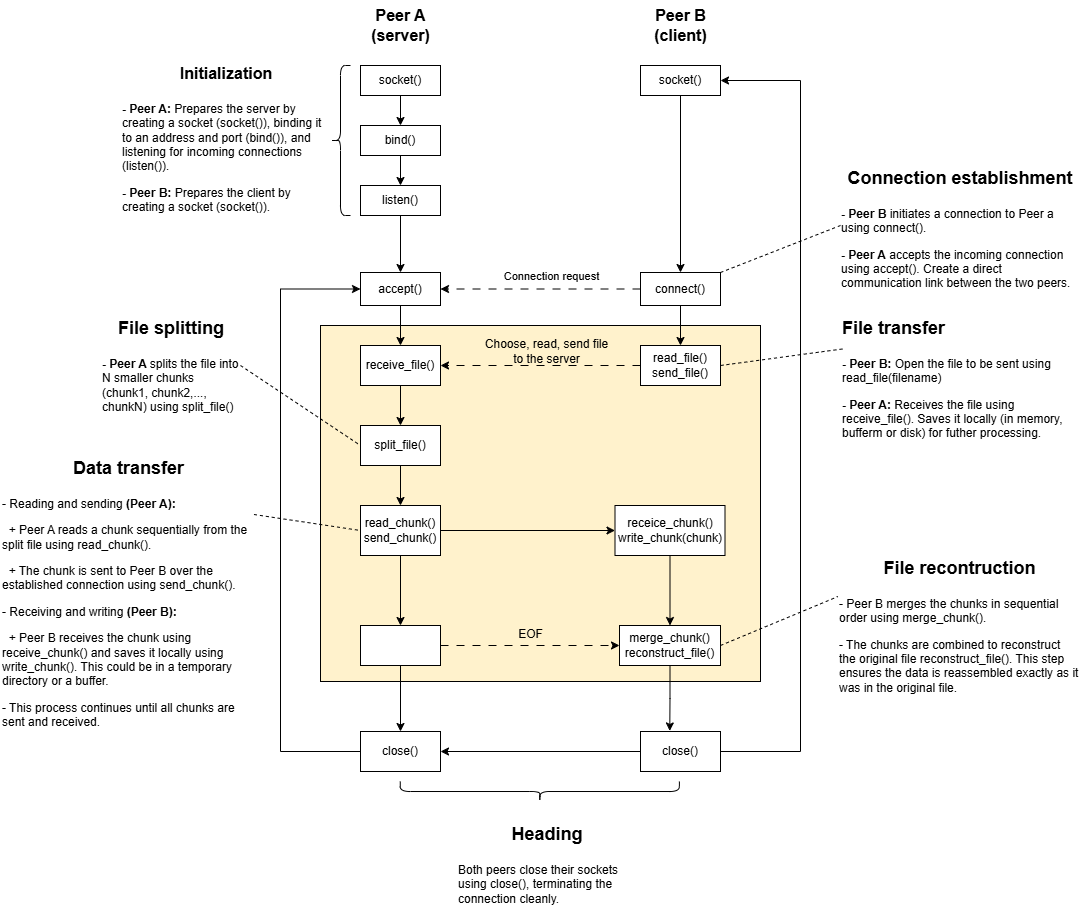
\includegraphics[width=\textwidth]{A-P2P-file-sharing-application-system.png}
    \caption{Illustration of Peer-to-Peer Network File Transfer Process}
    \label{fig:p2p-transfer}
\end{figure}
